\documentclass[sigconf,anonymous,review]{acmart}

\settopmatter{printacmref=false}
\setcopyright{none}
\renewcommand\footnotetextcopyrightpermission[1]{}
\pagestyle{plain}

\usepackage{booktabs}
\usepackage{graphicx}
\usepackage{tabularx}
\usepackage{multirow}
\usepackage{tikz}
\usetikzlibrary{arrows.meta,positioning,shapes.geometric}

\acmConference[AAMAS '26]{The 25th International Conference on Autonomous Agents and Multiagent Systems}{May 25--29, 2026}{Paphos, Cyprus}
\acmYear{2026}
\acmISBN{}
\acmDOI{}

\title{Verifiable Multi-Agent Reasoning for LLM Agents in Zero-Communication Mixed-Motive Games}

\begin{document}

\begin{abstract}
Large language model agents are increasingly evaluated in multi-agent decision settings, but final outcomes and fluent explanations do not guarantee valid reasoning. We study this problem in zero-communication mixed-motive games, where agents must cooperate with partners and compete against opponents without directly exchanging intentions or private information. We propose a verifier-grounded framework for evaluating LLM agents at structured decision points. Each agent outputs a reasoning trace containing its selected action, team objective, partner belief, opponent belief, action rationale, and risk assessment. A rule-grounded verifier checks the trace against legal action constraints, public history, hidden-information discipline, and reasoning-action consistency. We instantiate the framework in Guandan, a four-player imperfect-information partnership card game with dynamic legal actions and action-only implicit signaling. In a 50-decision pilot using Kimi Code CLI outputs, provider-complete LLM runs still expose substantial structured-reasoning failures: the plain condition parses 26/50 traces, the candidate-constrained condition parses 32/50 traces, the ToM-prompted condition parses 36/50 traces with 1 hard verifier failure among parsed traces, and verifier revision parses 32/32 eligible traces while reducing hard verifier failures from 35 to 10. These results support verifier-grounded reasoning as a practical diagnostic layer for LLM agents in structured multi-agent environments, while leaving full-game outcome evaluation and verifier-component ablations as follow-up work.
\end{abstract}

\keywords{LLM agents, multi-agent reasoning, mixed-motive games, imperfect information, verifiable reasoning, Guandan}

\maketitle

\section{Introduction}

Large language model (LLM) agents are increasingly used as decision makers in multi-agent environments where success depends on reasoning about other agents. Prior work has evaluated LLMs in coordination games, cooperative imperfect-information games, and mixed-motive social settings, showing that language models can sometimes coordinate, explain, or adapt their behavior~\citep{agashe2023llmcoordination,ramesh2026hanabi,xie2026m3bench}. However, outcome scores and plausible natural-language explanations do not establish whether an agent's stated beliefs and rationale are consistent with the observable state, the rules of the environment, and its chosen action.

Zero-communication mixed-motive games expose this weakness in a particularly sharp form. In these games, agents must cooperate with partners and compete against opponents, but they cannot directly exchange intentions or private information. Any coordination must therefore be inferred from public actions such as passes, sacrifices, resource use, or lead transfers. A model that claims to protect its partner while taking an action that blocks the partner, or a model that asserts hidden cards as facts, may still produce a fluent explanation and may even win by chance. Outcome-only evaluation cannot distinguish strategic reasoning from lucky or inconsistent behavior.

We study this problem through Guandan, a four-player partnership card game with imperfect information, dynamic legal actions, and two-vs-two cooperation and competition. Guandan is not used here as a target for building the strongest possible game bot. Instead, it is used as a dense testbed for verifiable multi-agent reasoning: the game contains strict rule constraints that can be checked deterministically, public histories that constrain valid beliefs, and action-only implicit signals that require partner and opponent modeling.

This paper asks whether verifier-grounded reasoning reveals failures that fluent explanations hide and whether verifier feedback can improve structured reasoning. Our framework represents each turn as a decision point with public history, hand counts, legal candidate actions, and strategic tags. The LLM agent outputs a structured reasoning trace containing its selected action, partner belief, opponent belief, team objective, action rationale, risk assessment, and confidence. A rule-grounded verifier labels the trace along hard and soft dimensions, including action legality, table-beating validity, public-history consistency, hidden-information discipline, partner consistency, opponent consistency, and reasoning-action consistency.

The pilot compares plain prompting, candidate-constrained prompting, ToM-prompted reasoning, and verifier-revision prompting on 50 controlled Guandan decision points. Provider outputs are complete for all first-pass prompts, but structured reasoning remains brittle: the plain condition yields 26 parsed traces out of 50 outputs, the candidate-constrained condition yields 32 parsed traces out of 50, the ToM-prompted condition yields 36 parsed traces with 1 hard verifier failure among parsed traces, and verifier revision parses all 32 eligible revision traces while reducing hard verifier failures from 35 to 10. The current evidence is a decision-point reasoning pilot rather than a full-game outcome evaluation.

\section{Related Work}

LLM coordination benchmarks establish that language-model agents can be evaluated as decision makers in multi-agent settings. LLM-Coordination studies pure coordination games through Agentic Coordination and CoordinationQA tasks, including environment comprehension, theory-of-mind reasoning, joint planning, and an answer-verification ablation for Hanabi safety~\citep{agashe2023llmcoordination}. Recent Hanabi work goes further by evaluating LLMs at scale in an imperfect-information cooperative card game, collecting reasoning traces, multi-turn memory, and dense move-level utilities~\citep{ramesh2026hanabi}. These settings are close, so our contribution is not the existence of LLM coordination, game-agent verification, or card-game reasoning traces; the distinction is deterministic checking of structured traces in a team-vs-team mixed-motive game with dynamic legal actions and hidden-information discipline.

Process-aware mixed-motive evaluation is already an active area. M3-BENCH evaluates LLM social behavior across mixed-motive games using behavioral trajectory, reasoning process, and communication content analyses~\citep{xie2026m3bench}. Explanation work in mixed-motive games addresses inter-agent competition, cheap talk, and implicit communication by actions~\citep{aaai2025mixedexplain}. These studies are close to our motivation; our contribution is not that mixed-motive reasoning should be evaluated beyond outcomes, but a narrower rule-grounded verification target for structured LLM traces under dynamic legal action constraints.

Guandan AI has been studied as both a reinforcement-learning problem and an LLM-agent problem. DanZero targets strong Guandan play through self-play reinforcement learning~\citep{lu2022danzero}, while OpenGuanDan provides a large-scale imperfect-information benchmark with variable action spaces, mixed cooperation and competition, and support for LLM integration~\citep{openguandan2026}. The closest work, ToM-Guandan, evaluates LLM agents in Guandan under imperfect information, collaboration, and absence of communication; it further proposes Theory-of-Mind planning and an RL-based action recommender for the dynamic legal action list~\citep{yim2024tomguandan}. Therefore, this paper must not be framed as introducing Guandan, LLM Guandan agents, zero-communication Guandan, ToM prompting, or action-space reduction. Our distinct target is whether the reasoning trace that accompanies an action is verifiably consistent with game rules, public evidence, hidden-information discipline, and the selected action.

Structured and verifiable reasoning methods provide useful design patterns but do not directly solve this evaluation setting. CodeAgents turns multi-agent planning into modular pseudocode and describes the resulting plans as interpretable and verifiable~\citep{yang2025codeagents}. Strat-Reasoner treats LLM game output as reasoning paired with action and optimizes strategic reasoning in multi-agent games~\citep{he2026stratreasoner}, while ToolPoker evaluates poker reasoning traces and addresses knowing-doing gaps under hidden information with solver-assisted tool use~\citep{lin2026toolpoker}. Related reasoning-execution gap work in mobile-use agents also shows that reasoning-action consistency is a known diagnostic concern in agent evaluation~\citep{ma2025saydo}. Our contribution is a domain-specific verifier formulation: hard checks for legal action, table beating, public-history consistency, and hidden-information discipline, plus conservative soft checks for reason-action and team-objective consistency.

\begin{table*}[t]
\centering
\caption{Related-work positioning. The closest work supplies many surrounding pieces; our focus is rule-grounded trace verification in zero-explicit-communication, mixed-motive, dynamic-action team play.}
\label{tab:related}
\small
\begin{tabularx}{\textwidth}{lllllX}
\toprule
Work & Setting & Comm. & Reasoning Signal & Grounding & Dynamic Actions \\
\midrule
LLM-Coordination & coordination games & varies & coordination/ToM reasoning & LLM verification + scores & no \\
Hanabi LLM agents & cooperative Hanabi & clues & traces + utilities & game scoring + annotations & game-specific \\
M3-BENCH & mixed-motive games & mixed & process metrics & BTA/RPA/CCA & no Guandan verifier \\
ToM-Guandan & Guandan & none & ToM planning + performance & action recommender + scores & yes \\
OpenGuanDan & Guandan benchmark & API & agent performance & simulator metrics & yes \\
Strat-Reasoner & multi-agent games & interaction & trace + action & RL reward + CoT comparison & not Guandan-specific \\
ToolPoker & poker & opponent modeling & reasoning traces & solver / reasoning metrics & poker actions \\
This project & Guandan decisions & none & structured trace labels & rule-grounded verifier & yes \\
\bottomrule
\end{tabularx}
\end{table*}

\section{Method}

\subsection{Problem Setup}

Our method evaluates LLM agents at decision points rather than only at the end of a game. A decision point contains the acting player, public history, private hand, hand counts, current table lead, legal candidate actions, and strategic scenario tags. This representation makes the evaluation local enough to label precisely while preserving the partner and opponent context needed for mixed-motive reasoning.

Formally, let a decision point be \(d_t = (p_t, h_t, o_t, c_t, A_t, z_t)\), where \(p_t\) is the acting player, \(h_t\) is the public action history, \(o_t\) is the acting player's private observation, \(c_t\) is the current table context, \(A_t\) is the finite set of legal candidate actions, and \(z_t\) contains scenario tags derived only from public state. An agent returns a structured trace \(r_t\) and selected action \(a_t \in A_t\). The verifier maps \((d_t, r_t, a_t)\) to labels \(y_t\) and issues \(e_t\). Labels are decomposed into hard checks, which can be determined from rules and public/private-state boundaries, and soft checks, which conservatively score whether the stated objective and beliefs are consistent with available public evidence.

\subsection{Decision-Point Exporter}

The decision-point exporter converts a game state and its public timeline prefix into schema-valid records. For each exported turn, the exporter reconstructs the public history up to that point, records the current player's private hand, computes or attaches legal candidate actions, summarizes played cards, and tags the strategic scenario. This produces a standardized input object for all agent conditions, preventing different prompts from receiving incompatible state information.

The exporter deliberately keeps the unit of analysis smaller than a full game. Full games are valuable for measuring win rate, but they make it difficult to determine whether a single explanation is invalid because the action was illegal, the model relied on hidden cards, or the downstream trajectory happened to punish a reasonable decision. A local decision point keeps the verifier's evidence set explicit: public claims can be checked against \(h_t\), private claims can be checked against the allowed observation boundary \(o_t\), and action claims can be checked against \(A_t\) and the table context \(c_t\).

\subsection{Structured Reasoning Trace}

The structured reasoning trace forces the LLM to expose the parts of its multi-agent reasoning that can be checked. For each decision, the agent must output a selected action, team objective, partner belief, opponent belief, action rationale, risk assessment, and confidence. This design avoids relying on unconstrained free-form explanations and gives the verifier explicit fields to check.

Table~\ref{tab:trace-schema} summarizes the trace fields. The schema is intentionally not a long chain-of-thought transcript. It asks for decision-relevant commitments that can be audited: the action, the cooperative objective, beliefs about the partner and opponents, the rationale linking state to action, and the risk acknowledged by the agent. This design is useful for publication because it gives reviewers a concrete artifact to inspect and reproduce without requiring access to private hidden reasoning.

\begin{table*}[t]
\centering
\caption{Structured reasoning trace schema used by all LLM conditions. The verifier checks field-level commitments against the decision point instead of judging an unconstrained explanation.}
\label{tab:trace-schema}
\small
\begin{tabularx}{\textwidth}{lllX}
\toprule
Field & Type & Evidence Boundary & Verifier Use \\
\midrule
selected action & structured action id & legal candidate set \(A_t\) & action legality and table-beating checks \\
team objective & short categorical text & public state and team identity & team-objective and reason-action checks \\
partner belief & belief statement + evidence ids & public history only & partner consistency and public-history checks \\
opponent belief & belief statement + evidence ids & public history only & opponent consistency and hidden-information checks \\
action rationale & concise explanation & public state, private hand, and legal actions & reason-action consistency checks \\
risk assessment & concise risk statement & current table and hand counts & soft plausibility checks \\
confidence & scalar/category & trace self-report & analysis field; not used to pass hard checks \\
\bottomrule
\end{tabularx}
\end{table*}

\subsection{Rule-Grounded Verifier}

The verifier separates hard rule checks from soft strategic consistency checks. Hard checks include action legality, table-beating validity, public-history consistency, and hidden-information discipline. Soft checks include partner consistency, opponent consistency, team-objective validity, and reasoning-action consistency. Hard failures indicate that a trace cannot be valid under the game state. Soft failures are diagnostic rather than dispositive: they flag a mismatch between the trace and a conservative public-state interpretation, but they do not prove that the selected action is strategically dominated.

The hard and soft split is important for avoiding overclaiming. Action legality and table-beating validity are deterministic under the rules. Public-history consistency is deterministic once the trace cites a public event or public tag: the cited evidence either exists in \(h_t\) or it does not. Hidden-information discipline is also a hard boundary: the agent may reason probabilistically about unobserved cards, but it must not state another player's hidden cards as known facts unless the information is entailed by public play. By contrast, partner consistency and opponent consistency are soft because multiple strategic readings may be plausible from the same public sequence.

The verifier records issue codes rather than only binary pass/fail labels. Issue codes make the feedback auditable and make paired attribution possible. For example, an \texttt{UNKNOWN\_PUBLIC\_EVIDENCE} issue means that the trace cited evidence that is not present in the exported public history, while \texttt{HIDDEN\_INFO\_ASSERTED\_AS\_FACT} means that the trace described unobserved cards or private intentions as certain. The issue-code layer is useful because two traces can both fail the same label for different reasons, and revision can repair one issue while leaving another unresolved.

\begin{table*}[t]
\centering
\caption{Verifier label taxonomy. Hard labels identify rule or information-boundary violations; soft labels diagnose strategic plausibility without claiming optimality.}
\label{tab:label-taxonomy}
\small
\begin{tabularx}{\textwidth}{lllX}
\toprule
Label & Type & Input Evidence & Failure Meaning \\
\midrule
legalAction & hard & \(A_t\), selected action & the chosen action is not in the legal candidate set \\
beatsTable & hard & table context, action shape & the action cannot legally beat or respond to the current table \\
publicHistoryConsistent & hard & public event ids, scenario tags & the trace cites or relies on public evidence not present in \(h_t\) \\
hiddenInfoDisciplined & hard & private/public boundary & the trace asserts hidden cards or intentions as facts \\
partnerConsistent & soft & partner actions and public tags & partner belief omits or contradicts available public signals \\
opponentConsistent & soft & opponent actions and hand counts & opponent belief is weakly supported or over-specific \\
teamObjectiveValid & soft & team identity and situation tag & stated objective does not fit the cooperative situation \\
reasonActionConsistent & soft & selected action and rationale & explanation does not support the selected action \\
\bottomrule
\end{tabularx}
\end{table*}

\subsection{Verifier-Grounded Revision}

The verifier-in-the-loop scaffold uses verification as feedback before finalizing an action. The agent first produces a structured reasoning trace. The verifier returns hard failures and soft warnings. The agent then revises its trace and selected action under the constraint that hard failures should be resolved. The final trace is evaluated against the same verifier labels, allowing a controlled comparison between initial and revised reasoning.

Algorithm~\ref{alg:revision} describes the revision protocol. The key design choice is that the verifier does not choose an action for the LLM. It exposes a compact set of labels and issue codes, then asks the model to repair its own trace under the same decision state. This keeps the evaluation focused on whether verifier feedback improves the model's reasoning commitments rather than replacing the model with a rule-based actor.

\begin{figure*}[t]
\centering
\setlength{\fboxsep}{7pt}
\fbox{\begin{minipage}{0.92\columnwidth}
\textbf{Algorithm 1: Verifier-Grounded Revision}

\textbf{Input:} decision point \(d_t\), legal actions \(A_t\), LLM \(M\), verifier \(V\)

\begin{enumerate}
\item Prompt \(M\) with \(d_t\) and request a structured trace \(r_t^{0}\).
\item Parse \(r_t^{0}\). If parsing fails, record a schema failure and stop.
\item Run \(V(d_t, r_t^{0})\) to obtain labels and issue codes.
\item If revision is enabled, prompt \(M\) with \(d_t\), \(r_t^{0}\), and verifier feedback.
\item Parse the revised trace \(r_t^{1}\); record a revision parse failure if needed.
\item Run \(V(d_t, r_t^{1})\) and compare labels with the initial trace on the paired decision id.
\end{enumerate}

\textbf{Output:} initial labels, revised labels, parse status, and paired deltas.
\end{minipage}}
\caption{Verifier-grounded revision protocol. Revision is evaluated only on traces that are parseable before revision, so parse failures outside the eligible subset remain an explicit reliability issue.}
\label{alg:revision}
\end{figure*}

\begin{figure*}[t]
\centering
\resizebox{\textwidth}{!}{%
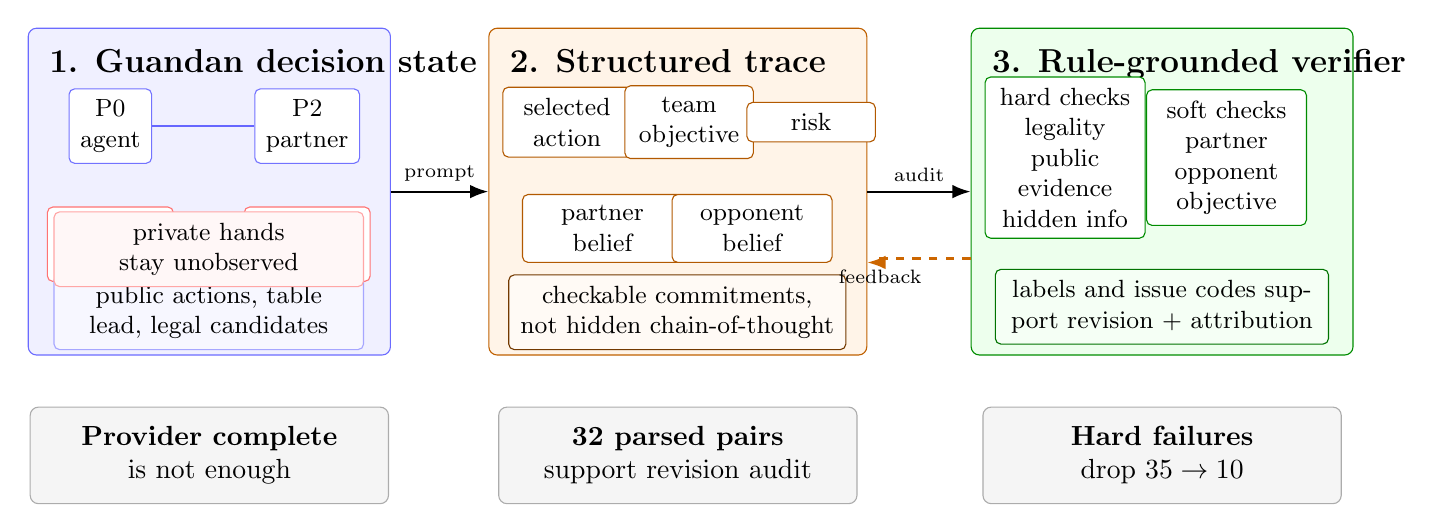
\begin{tikzpicture}[
  font=\normalsize,
  box/.style={draw, rounded corners=3pt, align=left, inner sep=7pt},
  state/.style={box, fill=blue!6, draw=blue!58, minimum width=4.6cm, minimum height=4.15cm},
  trace/.style={box, fill=orange!9, draw=orange!75!black, minimum width=4.8cm, minimum height=4.15cm},
  verifier/.style={box, fill=green!7, draw=green!55!black, minimum width=4.85cm, minimum height=4.15cm},
  evidence/.style={box, fill=gray!8, draw=gray!65, align=center, minimum width=4.55cm, minimum height=1.02cm},
  mini/.style={draw, rounded corners=2pt, align=center, font=\small, inner sep=4pt},
  arrow/.style={-Latex, thick},
  feedback/.style={-Latex, thick, dashed, draw=orange!80!black},
  title/.style={anchor=north west, font=\bfseries\large}
]
\node[state] (s) at (0,0) {};
\node[title] at ([xshift=0.15cm,yshift=-0.15cm]s.north west) {1. Guandan decision state};
\node[mini, fill=white, draw=blue!55] (p0) at ([xshift=1.05cm,yshift=-1.25cm]s.north west) {P0\\agent};
\node[mini, fill=white, draw=blue!55] (p2) at ([xshift=3.55cm,yshift=-1.25cm]s.north west) {P2\\partner};
\node[mini, fill=white, draw=red!55] (p1) at ([xshift=1.05cm,yshift=-2.75cm]s.north west) {P1\\opponent};
\node[mini, fill=white, draw=red!55] (p3) at ([xshift=3.55cm,yshift=-2.75cm]s.north west) {P3\\opponent};
\draw[thick, blue!60] (p0) -- (p2);
\draw[thick, red!50] (p1) -- (p3);
\node[mini, fill=blue!3, draw=blue!35, text width=3.65cm] at ([xshift=2.3cm,yshift=0.55cm]s.south west) {public actions, table lead, legal candidates};
\node[mini, fill=red!3, draw=red!35, text width=3.65cm] at ([xshift=2.3cm,yshift=1.35cm]s.south west) {private hands stay unobserved};

\node[trace] (r) at (5.95,0) {};
\node[title] at ([xshift=0.15cm,yshift=-0.15cm]r.north west) {2. Structured trace};
\node[mini, fill=white, draw=orange!70!black, text width=1.35cm] at ([xshift=1.0cm,yshift=-1.2cm]r.north west) {selected action};
\node[mini, fill=white, draw=orange!70!black, text width=1.35cm] at ([xshift=2.55cm,yshift=-1.2cm]r.north west) {team objective};
\node[mini, fill=white, draw=orange!70!black, text width=1.35cm] at ([xshift=4.1cm,yshift=-1.2cm]r.north west) {risk};
\node[mini, fill=white, draw=orange!70!black, text width=1.75cm] at ([xshift=1.45cm,yshift=-2.55cm]r.north west) {partner belief};
\node[mini, fill=white, draw=orange!70!black, text width=1.75cm] at ([xshift=3.35cm,yshift=-2.55cm]r.north west) {opponent belief};
\node[mini, fill=orange!4, draw=orange!45!black, text width=4.0cm] at ([xshift=2.4cm,yshift=0.55cm]r.south west) {checkable commitments, not hidden chain-of-thought};

\node[verifier] (v) at (12.1,0) {};
\node[title] at ([xshift=0.15cm,yshift=-0.15cm]v.north west) {3. Rule-grounded verifier};
\node[mini, fill=white, draw=green!55!black, text width=1.75cm] at ([xshift=1.2cm,yshift=-1.65cm]v.north west) {hard checks\\legality\\public evidence\\hidden info};
\node[mini, fill=white, draw=green!55!black, text width=1.75cm] at ([xshift=3.25cm,yshift=-1.65cm]v.north west) {soft checks\\partner\\opponent\\objective};
\node[mini, fill=green!4, draw=green!45!black, text width=3.95cm] at ([xshift=2.43cm,yshift=0.62cm]v.south west) {labels and issue codes support revision + attribution};

\draw[arrow] (s.east) -- node[above, font=\scriptsize] {prompt} (r.west);
\draw[arrow] (r.east) -- node[above, font=\scriptsize] {audit} (v.west);
\draw[feedback] ([yshift=-0.85cm]v.west) -- ++(-1.15,0) |- node[pos=0.2, below, font=\scriptsize] {feedback} ([yshift=-0.9cm]r.east);

\node[evidence] at (0,-3.35) {\textbf{Provider complete}\\is not enough};
\node[evidence] at (5.95,-3.35) {\textbf{32 parsed pairs}\\support revision audit};
\node[evidence] at (12.1,-3.35) {\textbf{Hard failures}\\drop \(35 \rightarrow 10\)};
\end{tikzpicture}
}
\caption{Verifier-grounded multi-agent reasoning pipeline. A zero-communication Guandan decision point exposes public actions, legal candidates, and private information boundaries; the LLM returns a structured trace; the verifier checks hard rule/information constraints and soft strategic consistency, then feeds issue codes into paired revision and attribution.}
\label{fig:pipeline}
\end{figure*}

\section{Experiments}

\subsection{Research Questions}

The experiments test whether verifier-grounded reasoning provides information beyond provider completion and fluent explanations. We ask three questions in the current pilot: whether LLM agents produce schema-valid verifiable reasoning traces, whether candidate constraints reduce verifier-visible failures, and whether verifier feedback improves reasoning reliability on traces that are eligible for revision. Figure~\ref{fig:pipeline} summarizes the pipeline from decision point to paired attribution.

\subsection{Benchmark Construction}

The benchmark consists of Guandan decision points generated from controlled game states. Each decision point includes public history, acting player, team identity, hand counts, current table lead, legal candidate actions, inference summaries, and strategic scenario tags. The repository currently contains a 50-decision pilot split and a 500-decision full-evaluation split. The pilot covers five scenario tags: lead opening, follow beat-or-pass, partner near finish, opponent near finish, and endgame race. The full split is retained as a local follow-up target; the current paper reports the cost-controlled pilot.

The pilot is designed as a diagnostic sample rather than a claim of environment-wide performance. Its purpose is to test whether the pipeline can expose concrete reasoning failures under controlled states, produce paired before/after labels, and generate publication-grade evidence tables. The 500-decision split is reserved for the next empirical stage because it requires a larger provider budget and stronger baseline coverage before the paper can make broader robustness claims.

\subsection{Conditions and Baselines}

We compare six reported artifact rows. Two deterministic baselines, \textsc{heuristic-legal-first} and \textsc{strategic-heuristic}, validate the local harness and verifier. The plain LLM receives the game state and outputs a reasoning trace and action. The candidate-constrained LLM is additionally shown the verifier-provided legal candidate list. The ToM-prompted LLM receives an explicit checklist for partner intent, opponent intent, and counterfactual candidate comparison under the same trace schema. The verifier-revision condition receives the candidate trace and verifier feedback, then produces a revised trace.

The deterministic baselines are not intended to be strong Guandan players. They serve as harness checks: if a legal-action heuristic failed legality or hidden-information labels, the exporter or verifier would be suspect. The LLM rows test increasingly structured interaction with the same decision state. The plain condition measures whether the model can infer the output contract and state constraints from the prompt. The candidate-constrained condition removes ambiguity about legal actions but still requires valid beliefs and rationale. The ToM-prompted condition asks the model to explicitly reason about partner intent, opponent intent, and counterfactual candidate actions under the same trace schema. The verifier-revision condition tests whether explicit feedback repairs the trace on paired decision ids.

\subsection{Metrics}

We report four metric families. Provider completion measures whether the external model returns an output for the prompt. Parse yield measures whether the output satisfies the structured trace schema. Hard verifier failures count violations of deterministic constraints: legal action, table beating, public-history consistency, and hidden-information discipline. Soft verifier burden counts fail plus unknown labels for strategic consistency dimensions, reported descriptively rather than as a correctness verdict.

This metric design separates three failure modes that are often conflated in LLM-agent evaluations. A provider-complete response can still be unusable if it is not parseable. A parseable response can still be invalid if it violates the rules or the information boundary. A trace that passes hard checks can still be strategically weak if its partner or opponent beliefs are poorly supported. The pilot therefore treats reasoning reliability as a layered diagnostic target rather than a single win-rate number.

\subsection{End-to-End Failure Accounting}

Before comparing verifier labels, we account for which outputs are eligible for each metric. This accounting matters because revision is only meaningful for traces that can be parsed before revision. Table~\ref{tab:accounting} separates provider completion, parse yield, revision eligibility, and hard verifier failures. The plain, candidate-constrained, and ToM-prompted prompts each receive 50 provider outputs, but many outputs fail the structured schema. The verifier-revision condition is therefore evaluated on 32 paired candidate traces, while the 18 unparseable candidate outputs remain counted as end-to-end failures outside the paired analysis.

\begin{table}[t]
\centering
\caption{End-to-end accounting for the 50-decision pilot. Revision results are paired only on candidate traces that were parseable before revision.}
\label{tab:accounting}
\scriptsize
\begin{tabular}{lrrrr}
\toprule
Condition & Outputs & Parsed & Excluded & Hard Fail. \\
\midrule
plain LLM & 50 & 26 & 24 & 26 \\
candidate constrained & 50 & 32 & 18 & 35 \\
ToM prompted & 50 & 36 & 14 & 1 \\
ToM + schema repair & 50 & 49 & 1 & 1 \\
verifier revision & 32 & 32 & 0 & 10 \\
\bottomrule
\end{tabular}
\end{table}

This table prevents a misleading reading of the revision result. The paired verifier denominator is 32 because only those decision ids have both pre-revision and post-revision traces; end-to-end reliability is still measured over 50 prompts. Thus, verifier feedback repairs many hard failures when a candidate trace is already parseable, but it does not make the full candidate condition reliable. Figure~\ref{fig:tom-schema-flow} gives the corresponding flow for the ToM schema-repair ablation.

\begin{figure}[t]
\centering
\resizebox{\columnwidth}{!}{%
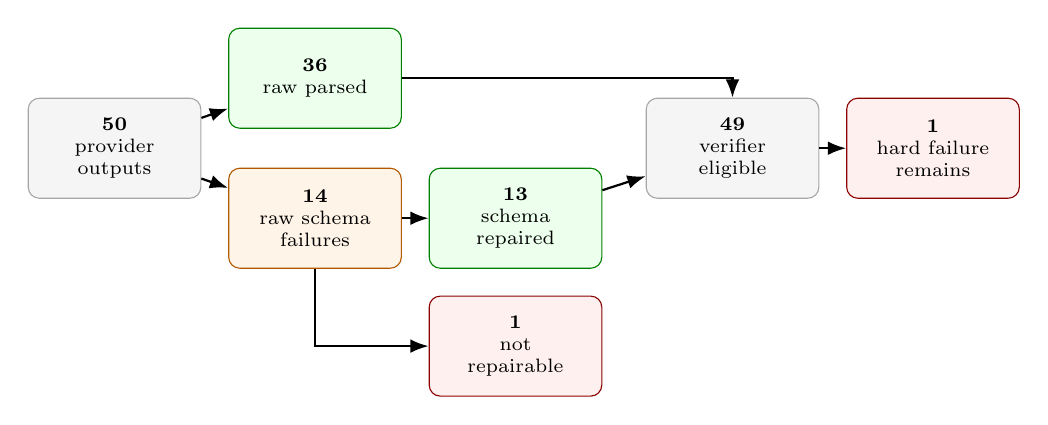
\begin{tikzpicture}[
  node distance=0.34cm,
  flowbox/.style={draw, rounded corners, align=center, text width=0.78in, minimum height=0.5in, font=\scriptsize, inner sep=3pt},
  good/.style={flowbox, fill=green!7, draw=green!50!black},
  warn/.style={flowbox, fill=orange!9, draw=orange!70!black},
  bad/.style={flowbox, fill=red!6, draw=red!55!black},
  neutral/.style={flowbox, fill=gray!8, draw=gray!70},
  arrow/.style={-Latex, thick}
]
\node[neutral] (out) {\textbf{50}\\provider\\outputs};
\node[good, right=of out, yshift=0.35in] (raw) {\textbf{36}\\raw parsed};
\node[warn, right=of out, yshift=-0.35in] (fail) {\textbf{14}\\raw schema\\failures};
\node[good, right=of fail] (repair) {\textbf{13}\\schema\\repaired};
\node[bad, below=of repair] (unrep) {\textbf{1}\\not\\repairable};
\node[neutral, right=0.55cm of repair, yshift=0.35in] (elig) {\textbf{49}\\verifier\\eligible};
\node[bad, right=of elig] (hard) {\textbf{1}\\hard failure\\remains};
\draw[arrow] (out) -- (raw);
\draw[arrow] (out) -- (fail);
\draw[arrow] (fail) -- (repair);
\draw[arrow] (fail) |- (unrep);
\draw[arrow] (raw) -| (elig);
\draw[arrow] (repair) -- (elig);
\draw[arrow] (elig) -- (hard);
\end{tikzpicture}
}
\caption{ToM schema-repair flow. The repair layer preserves the selected action, recovers 13 non-conforming outputs, leaves one output unrepaired, and keeps the hard verifier failure visible.}
\label{fig:tom-schema-flow}
\end{figure}

\subsection{Main Pilot Results}

\begin{figure*}[t]
\centering
\resizebox{0.96\textwidth}{!}{%
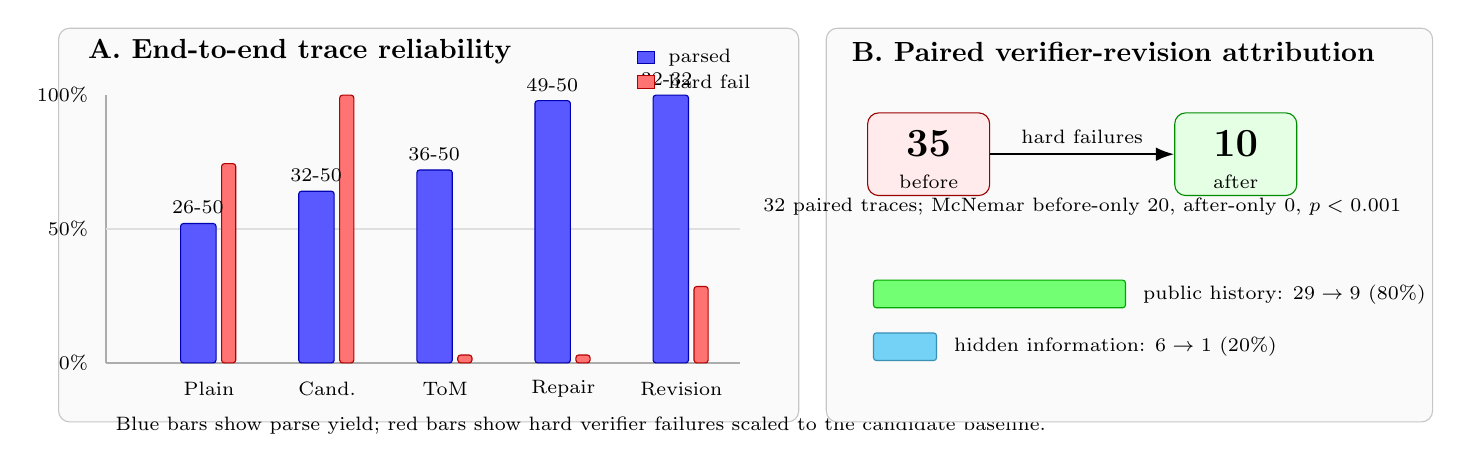
\begin{tikzpicture}[
  font=\small,
  panel/.style={draw=gray!45, rounded corners=4pt, fill=gray!4},
  axis/.style={draw=gray!65, thick},
  parsebar/.style={fill=blue!65, draw=blue!70!black},
  hardbar/.style={fill=red!55, draw=red!70!black},
  good/.style={fill=green!10, draw=green!55!black, rounded corners=4pt},
  bad/.style={fill=red!8, draw=red!60!black, rounded corners=4pt},
  arrow/.style={-Latex, thick},
  lab/.style={font=\scriptsize, align=center}
]
\node[panel, minimum width=9.4cm, minimum height=5.0cm] (a) at (0,0) {};
\node[anchor=west, font=\bfseries] at (-4.45,2.2) {A. End-to-end trace reliability};
\draw[axis] (-4.1,-1.75) -- (3.95,-1.75);
\draw[axis] (-4.1,-1.75) -- (-4.1,1.65);
\node[anchor=east, lab] at (-4.2,1.65) {100\%};
\node[anchor=east, lab] at (-4.2,-0.05) {50\%};
\node[anchor=east, lab] at (-4.2,-1.75) {0\%};
\draw[gray!25] (-4.1,-0.05) -- (3.95,-0.05);

\foreach \x/\h/\hard/\name/\count in {
  -3.15/1.77/2.53/Plain/26-50,
  -1.65/2.18/3.40/Cand./32-50,
  -0.15/2.45/0.10/ToM/36-50,
   1.35/3.33/0.10/Repair/49-50,
   2.85/3.40/0.97/Revision/32-32
}{
  \draw[parsebar, rounded corners=1pt] (\x,-1.75) rectangle ++(0.45,\h);
  \draw[hardbar, rounded corners=1pt] (\x+0.52,-1.75) rectangle ++(0.18,\hard);
  \node[lab] at (\x+0.22,\h-1.55) {\count};
  \node[lab] at (\x+0.36,-2.08) {\name};
}
\draw[parsebar] (2.65,2.05) rectangle ++(0.22,0.16);
\node[anchor=west, lab] at (2.92,2.13) {parsed};
\draw[hardbar] (2.65,1.74) rectangle ++(0.22,0.16);
\node[anchor=west, lab] at (2.92,1.82) {hard fail};
\node[anchor=west, lab] at (-4.1,-2.55) {Blue bars show parse yield; red bars show hard verifier failures scaled to the candidate baseline.};

\node[panel, minimum width=7.7cm, minimum height=5.0cm] (b) at (8.9,0) {};
\node[anchor=west, font=\bfseries] at (5.25,2.2) {B. Paired verifier-revision attribution};
\node[bad, minimum width=1.55cm, minimum height=1.05cm] (before) at (6.35,0.9) {};
\node at (6.35,1.04) {\Large\textbf{35}};
\node[lab] at (6.35,0.55) {before};
\node[good, minimum width=1.55cm, minimum height=1.05cm] (after) at (10.25,0.9) {};
\node at (10.25,1.04) {\Large\textbf{10}};
\node[lab] at (10.25,0.55) {after};
\draw[arrow] (before) -- node[above, lab] {hard failures} (after);
\node[lab] at (8.30,0.23) {32 paired traces; McNemar before-only 20, after-only 0, \(p<0.001\)};

\draw[fill=green!55, draw=green!65!black, rounded corners=1pt] (5.65,-1.05) rectangle ++(3.2,0.35);
\node[anchor=west, lab] at (8.95,-0.88) {public history: \(29 \rightarrow 9\) (80\%)};
\draw[fill=cyan!55, draw=cyan!70!black, rounded corners=1pt] (5.65,-1.72) rectangle ++(0.8,0.35);
\node[anchor=west, lab] at (6.55,-1.55) {hidden information: \(6 \rightarrow 1\) (20\%)};
\end{tikzpicture}
}
\caption{Main pilot results. Parse yield improves from 26/50 for plain LLM prompting to 36/50 under ToM prompting and 49/50 after deterministic ToM schema repair. On the 32 paired candidate traces, verifier revision reduces hard verifier failures from 35 to 10; 80\% of the hard-failure-count drop comes from public-history consistency and 20\% from hidden-information discipline.}
\label{fig:main-pilot-results}
\end{figure*}

The current pilot metrics summary is generated from experiment artifacts. The two deterministic baselines parse 50/50 traces and have zero hard failures, confirming that the schemas, verifier, and table generation path are internally consistent. The plain LLM condition has complete provider outputs for 50/50 prompts but only 26 parsed traces, with 24 schema parse failures and 26 hard verifier failures. The candidate-constrained condition also has complete provider outputs for 50/50 prompts, improves parse yield to 32 traces, but still has 35 hard verifier failures. The ToM-prompted condition has complete provider outputs for 50/50 prompts, parses 36 traces, and has 1 hard verifier failure among parsed traces. A deterministic schema-repair ablation preserves the ToM-selected action and raises ToM parse yield to 49/50 while leaving the hard failure count at 1. The verifier-revision condition is generated only for the 32 parsed candidate traces; it parses 32/32 revised traces and reduces hard failures to 10 (Figure~\ref{fig:main-pilot-results}).

Figure~\ref{fig:main-pilot-results} also shows why prompt structure changes the visible failure profile. Showing legal candidates makes action parsing easier and keeps legal-action failures at zero among parsed candidate traces, but it exposes more reasoning commitments to the verifier. The ToM prompt improves parse yield and sharply reduces hard verifier failures among parsed traces, while still leaving 14 outputs outside the structured trace schema. The result should therefore be read as diagnostic evidence about reasoning-trace reliability, not as a claim that ToM prompting solves strategic play.

The ToM failure analysis separates schema compliance from reasoning validity. Of the 14 ToM parse failures, 11 contain plausible reasoning inside a nested \texttt{reasoning} object but do not expose the required top-level trace fields, 2 miss required fields under other aliases, and 1 is a tool-call-like output. The schema-repair ablation confirms this diagnosis: 13 outputs are recoverable without changing \texttt{selectedActionId}, while the tool-call-like output remains unrepaired. Among the 49 repaired-or-passed-through ToM traces, the only hard verifier failure is still a hidden-information assertion. This pattern suggests that ToM prompting improves verifier-visible reasoning when the trace is parseable, but end-to-end reliability still needs schema-constrained decoding or a repair layer.

The main comparison shows that verifier revision reduces verifier-visible failures on the parsed candidate subset. Failure burden, defined as fail plus unknown, drops most strongly for public-history consistency, from 29 before revision to 9 after revision. Hidden-information burden drops from 6 to 1, partner consistency burden from 29 to 26, opponent consistency burden from 22 to 20, reasoning-action burden from 1 to 0, and team-objective burden from 19 to 18. Legal-action and table-beating burdens are already zero in the candidate traces and remain zero after revision.

\begin{table}[t]
\centering
\caption{Verifier-revision effect on the 32 eligible candidate traces. Burden is fail plus unknown; deltas are after minus before.}
\label{tab:revision}
\scriptsize
\begin{tabular}{lrrr}
\toprule
Label & Before & After & Delta \\
\midrule
legalAction & 0 & 0 & 0 \\
beatsTable & 0 & 0 & 0 \\
publicHistoryConsistent & 29 & 9 & -20 \\
hiddenInfoDisciplined & 6 & 1 & -5 \\
partnerConsistent & 29 & 26 & -3 \\
opponentConsistent & 22 & 20 & -2 \\
reasonActionConsistent & 1 & 0 & -1 \\
teamObjectiveValid & 19 & 18 & -1 \\
\bottomrule
\end{tabular}
\end{table}

To address whether the revision effect is concentrated in verifier-grounded reasoning labels rather than only output formatting, we add a paired verifier-attribution analysis over the same 32 eligible candidate traces. Hard failures drop from 35 to 10, with a paired bootstrap 95\% confidence interval of [-32, -18] for the hard-failure-count delta. At the decision level, hard-failure presence drops from 29 to 9 decisions, with 20 before-only failures and 0 after-only failures under a McNemar exact test. Component attribution shows that 80\% of the hard-failure-count drop comes from public-history consistency and 20\% from hidden-information discipline.

\subsection{Paired Statistical Analysis}

The paired analysis uses decision ids as the resampling unit. For hard-failure-count deltas, we resample the 32 paired decision ids with replacement and recompute the after-minus-before delta. This bootstrap interval is descriptive because the pilot is not a randomized benchmark sample from a fully specified population. For decision-level hard-failure presence, we use the paired before-only and after-only counts, which directly test whether failures disappear more often than they appear under revision. The observed table has 20 before-only hard-failure decisions and 0 after-only hard-failure decisions, yielding a McNemar exact p-value below 0.001.

We report this paired analysis to make the revision claim narrower and more defensible. A raw before/after count could be confounded by different decision sets, parsing filters, or repeated examples. Pairing ensures that every reported revision delta compares the same decision id before and after verifier feedback. The remaining weakness is subset selection: the paired set excludes the 18 candidate outputs that did not parse before revision. This is why the paper reports both end-to-end accounting and paired attribution instead of only the more favorable paired result.

\subsection{Qualitative Case Pack}

The qualitative case pack illustrates what the attribution numbers mean operationally. In one public-history repair, the original trace selected the same legal low-single action before and after revision, but its partner evidence used natural-language claims not present as public evidence ids and omitted the public partner-near-finish tag. The revised trace keeps the action and rationale stable while replacing unsupported evidence with a public event id and explicitly hedging the partner's hidden cards. In one hidden-information repair, the first trace combines an unsupported public-evidence citation with an assertion about opponents' cards. The revision keeps the selected action, rewrites the rationale, and changes the opponent belief from asserted holdings to public hand-count reasoning. The case pack also includes a remaining public-history failure after revision and a parse failure outside the revision subset, where the raw candidate output contains only a compact action and free-form reasoning field.

\begin{table*}[t]
\centering
\caption{Qualitative verifier-attribution case pack. Cases are selected from the generated attribution artifact to illustrate repaired, unrepaired, and out-of-subset failures.}
\label{tab:case-pack}
\scriptsize
\begin{tabularx}{\textwidth}{p{0.16\textwidth}p{0.21\textwidth}p{0.07\textwidth}p{0.23\textwidth}X}
\toprule
Case & Decision id & Action changed & Key label transition & Interpretation \\
\midrule
public-history repair & pilot-e1-002-turn-1-player-0 & no & publicHistory: fail to pass; partner: fail to pass & revision replaces unsupported public-evidence claims and adds the omitted partner-near-finish public tag \\
hidden-info repair & pilot-e1-013-turn-1-player-0 & no & publicHistory: fail to pass; hiddenInfo: fail to pass & revision changes asserted opponent holdings into public hand-count reasoning \\
remaining hard failure & pilot-e1-004-turn-1-player-0 & no & publicHistory: fail to fail & revision keeps an unknown public-evidence reference, showing verifier feedback does not guarantee repair \\
parse failure outside subset & pilot-e1-000-turn-1-player-0 & n/a & n/a & candidate output does not match the trace schema, so it is excluded from paired revision but counted as end-to-end unreliability \\
\bottomrule
\end{tabularx}
\end{table*}

\subsection{Reproducibility and Provenance}

The reported pilot is tied to local artifacts rather than hand-copied spreadsheet values. Provider outputs, parsed traces, verifier labels, paired attribution summaries, generated Markdown tables, the reproducibility manifest, the local pipeline report, and the AAMAS LaTeX draft are all stored under the repository's research directory. The local pipeline regenerates the paper-facing reports and checks that unresolved source, uncertainty, experiment, submission-blocking, or author-decision placeholders are absent from the submission artifacts.

\begin{table}[t]
\centering
\caption{Current provenance boundary for the AAMAS draft. The paper reports the pilot values only where an artifact exists locally.}
\label{tab:provenance}
\scriptsize
\begin{tabularx}{\columnwidth}{lX}
\toprule
Artifact & Role \\
\midrule
pilot experiment outputs & provider responses, parse status, verifier labels \\
reasoning reliability table & main 50-decision pilot summary \\
verifier attribution report & paired 32-trace before/after analysis \\
local pipeline report & end-to-end regeneration status for research artifacts \\
reproducibility manifest & file inventory and checksums for durable outputs \\
AAMAS LaTeX draft & compiled paper source and rendered PDF \\
\bottomrule
\end{tabularx}
\end{table}

\subsection{Full-Split Sanity Check}

To verify that the evaluation substrate scales beyond the 50-decision pilot, we run the two deterministic baselines on the 500-decision full split. This experiment does not use an LLM and does not test the paper's main revision claim. Its purpose is narrower: it checks whether the full decision-point split, trace schema, baseline trace generator, and verifier can produce complete artifacts without hard verifier failures under controlled non-LLM traces.

\begin{table}[t]
\centering
\caption{Full-split deterministic baseline sanity check. These rows validate the 500-decision substrate and verifier plumbing; they are not LLM results.}
\label{tab:full-baseline}
\scriptsize
\begin{tabular}{lrrr}
\toprule
Baseline & Parsed & Hard Fail. & Hidden P/F/U \\
\midrule
legal-first & 500/500 & 0 & 500/0/0 \\
strategic heuristic & 500/500 & 0 & 500/0/0 \\
\bottomrule
\end{tabular}
\end{table}

The full-split sanity check matters for the AAMAS submission path because it separates two risks. The first risk is infrastructure risk: the full split, schemas, and verifier may fail once scaled from 50 to 500 decisions. Table~\ref{tab:full-baseline} reduces this risk for deterministic traces. The second risk is model-reasoning risk: LLM traces may still fail to parse, cite unsupported public evidence, or assert hidden information. That risk remains open until a full-split LLM provider run is completed.

\subsection{Full-Evaluation Protocol}

The current pilot establishes that the verifier pipeline is operational and that paired revision can repair many hard reasoning failures. A full AAMAS submission should add a larger evaluation layer before making broader empirical claims. Table~\ref{tab:full-protocol} records the protocol that follows directly from the current artifacts. The key expansion is not only more prompts; it is a wider evidence package that tests whether verifier-grounded reasoning remains useful across more decision states, stronger prompting baselines, and component-removal variants.

\begin{table}[!t]
\centering
\caption{Protocol reserved for the full AAMAS empirical package. Rows describe required evidence before broad claims about robustness, generality, or strategic value.}
\label{tab:full-protocol}
\scriptsize
\begin{tabularx}{\columnwidth}{lX}
\toprule
Evaluation Layer & Required Evidence \\
\midrule
500-decision split & parse yield, hard failures, and soft burden beyond the 50-decision pilot \\
ToM-prompted LLM baseline & same verifier labels under a stronger reasoning-prompt baseline \\
Verifier-component ablation & paired deltas after removing label groups from revision feedback \\
Full-game rollout link & win rate and catastrophic-decision rate for verifier-valid traces \\
Human soft-label audit & agreement on partner/opponent consistency labels for sampled traces \\
\bottomrule
\end{tabularx}
\end{table}

This protocol also defines the next kill criteria. If the 500-decision split shows that revision mainly improves parse compliance but not public-history or hidden-information labels, the current contribution should be reframed as a formatting and schema-enforcement method. If component ablations show that nearly all gains come from exposing legal candidates, the verifier contribution is weaker than the current pilot suggests. Conversely, if public-history and hidden-information repairs persist under the larger split and remain paired after stronger baselines, the work becomes a stronger AAMAS candidate because it supports a general diagnostic claim rather than a small prompt anecdote.

\section{Discussion and Limitations}

\subsection{What the Verifier Establishes}

Verifier-grounded reasoning should be interpreted as diagnostic evidence rather than proof of strategic optimality. Hard labels can identify illegal actions, table-beating errors, public-history contradictions, and hidden-information hallucinations. Soft labels such as partner consistency and opponent consistency are more limited: they indicate whether the reasoning is plausible under the public state and selected objective, not whether the action is globally optimal.

The zero-communication setting is central to the contribution. When agents can communicate freely, reasoning quality can be evaluated through messages, negotiation, and explicit commitments. In Guandan-like settings, partners cannot directly reveal private cards or intentions, so action choices themselves become the coordination channel. This makes reasoning-action consistency a necessary diagnostic: if the action is the signal, the explanation must align with the signal.

This perspective also clarifies the difference between our verifier and an action recommender. An action recommender attempts to choose a high-value move. Our verifier asks a narrower question: given an action and an explanation, is the trace compatible with the rules, public evidence, hidden-information boundary, and stated team objective? This narrower target is easier to make deterministic, easier to reproduce, and less likely to conflate bad play with invalid reasoning.

\subsection{Threats to Validity}

Guandan is used as a compact testbed for imperfect information, dynamic legal actions, public histories, and mixed team objectives. The paper does not claim cross-game transfer. The paired attribution analysis shows that the hard-failure reduction is concentrated in public-history and hidden-information checks, but it is still measured only on the 32 candidate traces that were parseable and eligible for revision. The 18 unparseable candidate outputs remain an end-to-end reliability problem rather than a revision-success denominator.

Finally, LLM results are model- and prompt-sensitive. The pilot should therefore be read as a diagnostic pattern under a specified provider/client setting, not as a universal claim about all LLM agents. Future work should add additional model families, full-game outcome evaluation, component-removal ablations, and human annotation for a small subset of soft strategic labels.

The study also separates reasoning validity from downstream win rate. A stronger win-rate experiment would not by itself prove that explanations are grounded, and a grounded explanation does not guarantee the highest-value action. The next step is to test whether verifier-valid traces correlate with full-game outcomes, teammate compatibility, or reduced catastrophic decisions.

\subsection{Reviewer-Relevant Boundaries}

The closest likely reviewer objection is that verifier feedback might merely improve formatting. The paired attribution analysis partially addresses this by showing that the hard-failure reduction is concentrated in semantic verifier labels, especially public-history consistency and hidden-information discipline. However, the pilot does not yet prove that the model has learned a durable reasoning skill; it proves that, on paired eligible traces, explicit verifier feedback repairs many detectable invalid commitments. The paper therefore frames the result as evidence for a diagnostic layer and revision protocol, not as a final agent-training method.

Another likely objection is that the verifier depends on domain-specific rules. We view this as a feature of the first instantiation rather than a defect. The paper's general lesson is not that every game should use Guandan-specific issue codes, but that mixed-motive LLM-agent evaluation benefits from separating deterministic information-boundary checks from softer strategic plausibility checks. A future cross-domain version would need new exporters and rule checkers, while retaining the same trace and label philosophy.

\section{Conclusion}

This paper presents a verifier-grounded framework for evaluating LLM-agent reasoning in zero-communication mixed-motive games. In Guandan decision points, the framework converts each turn into a structured state, requires checkable commitments, and applies rule-grounded labels for legality, public-history consistency, hidden-information discipline, and reason-action consistency. The 50-decision pilot shows that provider-complete LLM outputs can still be brittle, while verifier revision reduces hard failures on the 32 eligible paired traces from 35 to 10. The core result is not a stronger card-playing bot, but a reproducible way to reveal and repair invalid reasoning commitments in a compact cooperative-competitive environment.

\bibliographystyle{ACM-Reference-Format}
\bibliography{../references}

\end{document}
